\subsection{Pseudo-Time Evolution of the Temperature Field}
\label{subsec:temperature_evolution}

The development of the temperature field during the numerical
solution is illustrated in Figure~\ref{fig:final_temperature}.
The sequence of temperature distributions shows the combined
effects of convection, thermal diffusion, and viscous
dissipation as the solution evolves from the initial condition
toward the steady state.

The effect of convection is evident from the deformation
of the temperature contours along the channel. Since the
prescribed parabolic velocity profile varies across the
channel height, fluid near the centreline is transported
downstream faster than fluid near the walls. This produces
a curved, approximately hyperbolic pattern in the
temperature distribution.

Viscous dissipation introduces a symmetric heating
contribution across the channel. This follows from the
squared wall-normal velocity gradient, which is symmetric
about the channel centreline and reaches its maximum
magnitude near the two walls. Consequently, the temperature
in the fluid cells adjacent to the lower wall initially
increases due to viscous heating. As the solution develops,
this local temperature increase is followed by a slight
decrease, as convective transport of relatively cooler
fluid from the inlet competes with the heating contribution.

The effect of thermal diffusion is particularly visible
in the downstream region of the channel. Heat is conducted
in the wall-normal direction from the warmer upper region
toward the cooler lower region, leading to a gradual
redistribution and smoothing of the temperature field
across the channel height.

Overall, the temperature evolution illustrates the
interaction between the three transport mechanisms and
their contributions to the resulting steady-state
temperature distribution.

\begin{figure}[htbp]
    \centering
    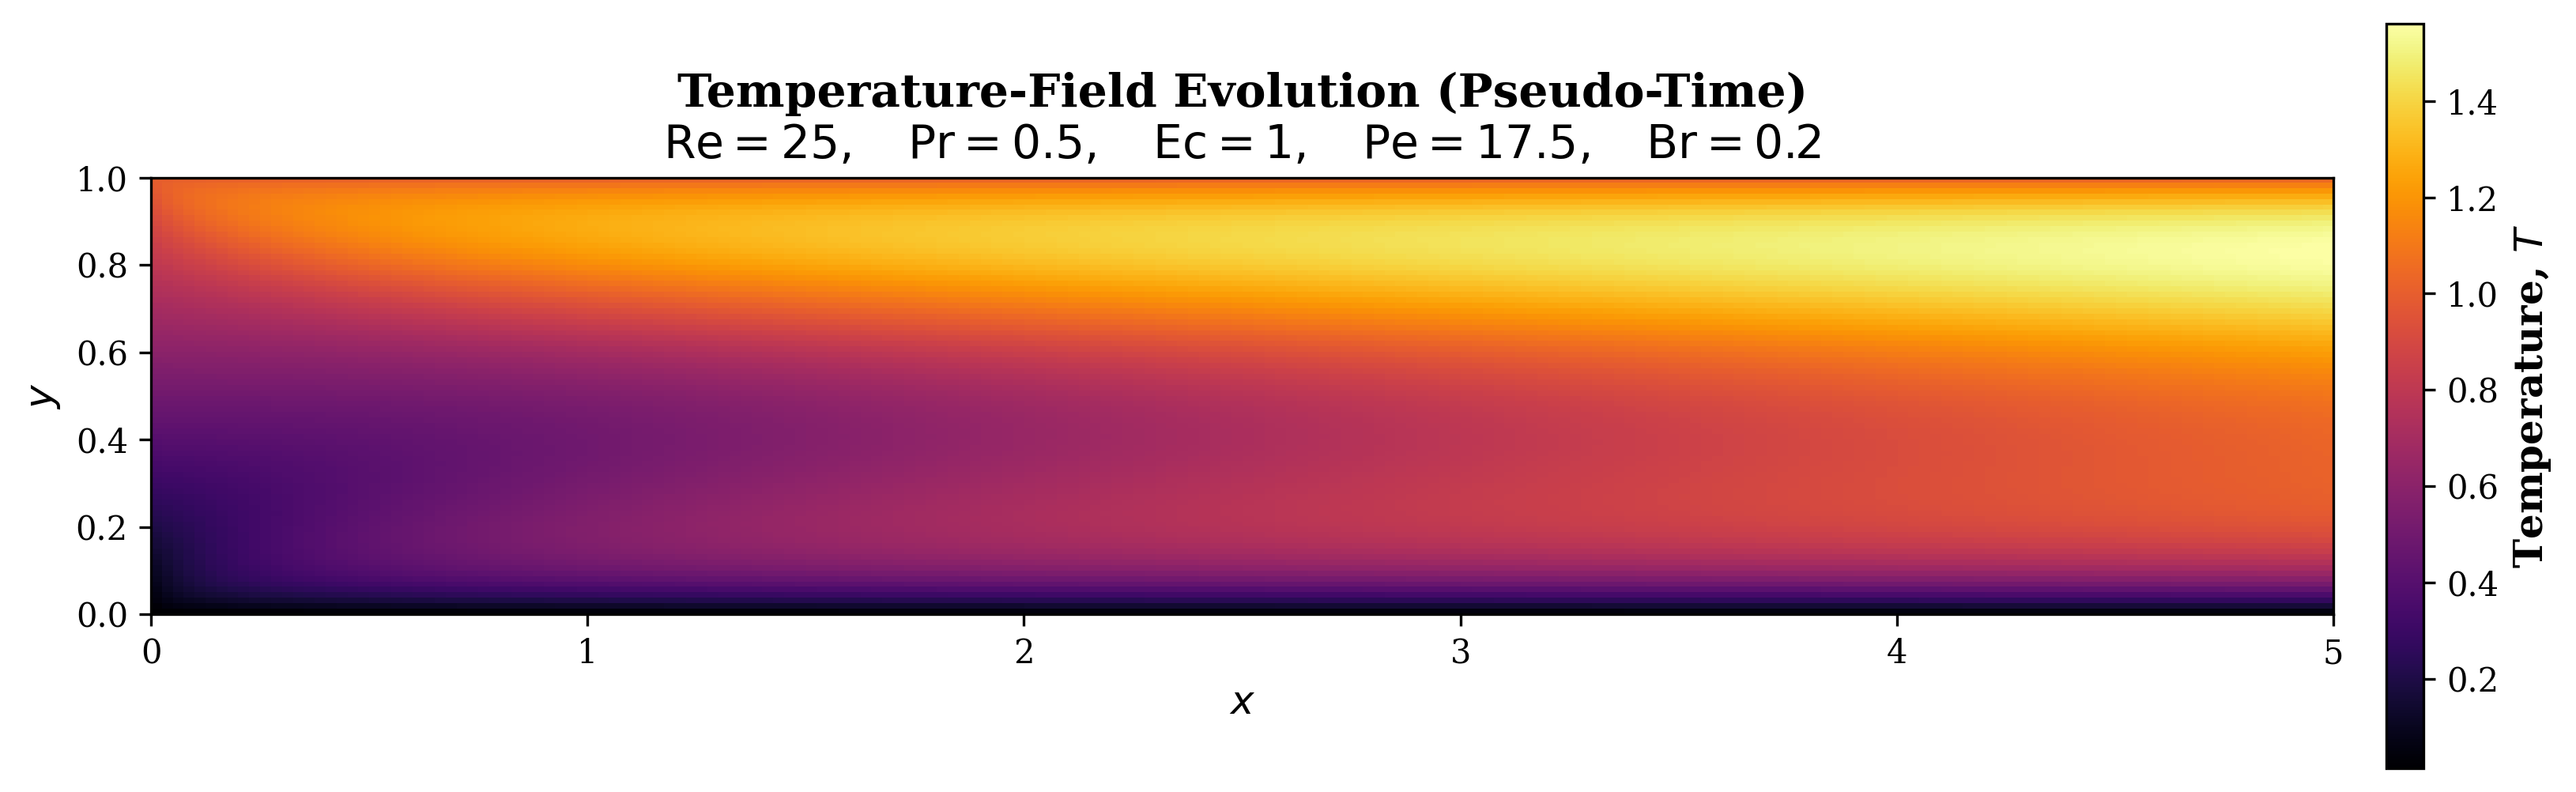
\includegraphics[width=0.85\textwidth]
    {figures/final_temperature.png}
    \caption{Representative temperature-field distribution
    during pseudo-time integration.}
    \label{fig:final_temperature}

    \vspace{0.2cm}
    \small
    \href{run:figures/temperature_evolution.gif}
    {Click here to view the complete temperature evolution
    animation (gif).}
\end{figure}